\subsection{User table}\label{subsec:user-table}

\texttt{
    CREATE TABLE public."user" \\
    ( \\
    id integer NOT NULL, \\
    name character varying(50) NOT NULL, \\
    email character varying(50) NOT NULL, \\
    created\_date character varying(50), \\
    updated\_date character varying(50), \\
    PRIMARY KEY (id), \\
    CONSTRAINT name\_unique UNIQUE (name), \\
    CONSTRAINT email\_unique UNIQUE (email) \\
    ); \\
    \\
    ALTER TABLE IF EXISTS public."user" \\
    OWNER to postgres; \\
}

\subsection{Event table}\label{subsec:event-table}

\texttt{
    CREATE TABLE public.event \\
    ( \\
    id integer NOT NULL,\\
    title character varying(50) NOT NULL,\\
    date character varying(50) NOT NULL,\\
    created\_date character varying(50),\\
    updated\_date character varying(50),\\
    PRIMARY KEY (id),\\
    CONSTRAINT title\_date UNIQUE (title, date)\\
    );\\
    \\
    ALTER TABLE IF EXISTS public.event\\
    OWNER to postgres;\\
}

\subsection{Ticket table}\label{subsec:ticket-table}

\texttt{
    CREATE TABLE public.ticket \\
    ( \\
    id integer NOT NULL,\\
    user\_id integer NOT NULL,\\
    event\_id integer NOT NULL,\\
    place integer NOT NULL,\\
    category character varying(30) NOT NULL,\\
    created\_date character varying(50),\\
    updated\_date character varying,\\
    PRIMARY KEY (id),\\
    CONSTRAINT unique\_event\_id\_place UNIQUE (event\_id, place),\\
    CONSTRAINT foreign\_key\_user\_id FOREIGN KEY (user\_id)\\
    REFERENCES public."user" (id) MATCH SIMPLE\\
    ON UPDATE NO ACTION\\
    ON DELETE NO ACTION\\
    NOT VALID,\\
    CONSTRAINT foreign\_key\_event\_id FOREIGN KEY (event\_id)\\
    REFERENCES public.event (id) MATCH SIMPLE\\
    ON UPDATE NO ACTION\\
    ON DELETE NO ACTION\\
    NOT VALID\\
    );\\
    \\
    ALTER TABLE IF EXISTS public.ticket\\
    OWNER to postgres;\\
}

\subsection{Database entity relations}\label{subsec:database-entity-relations}

\begin{figure}[h]
    \centering
    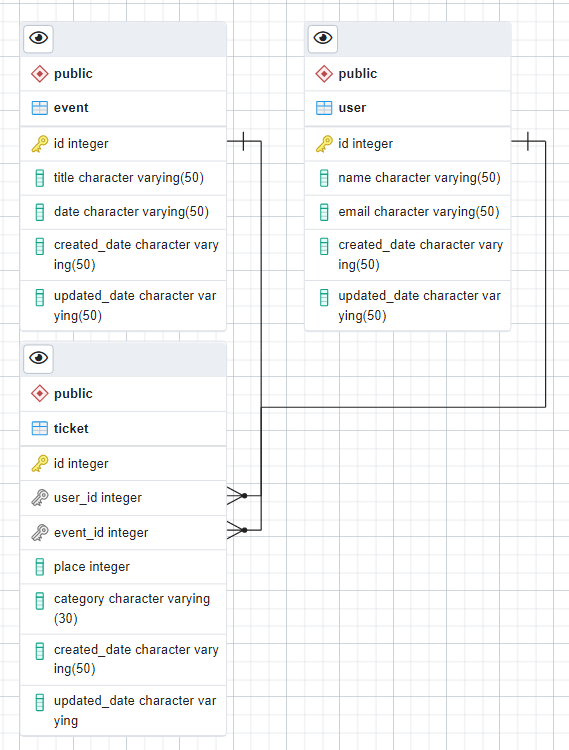
\includegraphics[width=0.8\textwidth]{images/database_relations}
    \caption{Entities relation in the database}
    \label{fig:db_relations}
\end{figure}

\subsection{Trigger for update time on UPDATE}\label{subsec:trigger-update-time}

Trigger function looks like:

\texttt{
    CREATE OR REPLACE FUNCTION public.set\_update\_time() \\
    RETURNS trigger \\
    LANGUAGE 'plpgsql' \\
    VOLATILE \\
    COST 100 \\
    AS \$BODY\$ \\
    BEGIN \\
    new.updated\_time = CURRENT\_TIME(2); \\
    RETURN new; \\
    END; \\
    \$BODY\$; \\
}

Trigger looks like:

\texttt{
    CREATE TRIGGER set\_update\_time\_on\_update \\
    BEFORE UPDATE OF id, name, email, created\_date, updated\_date \\
    ON public."user" \\
    FOR EACH ROW \\
    EXECUTE FUNCTION public.set\_update\_time(); \\
}

\subsection{Trigger for name validation}\label{subsec:trigger-name-validation}

Function to validate name:

\texttt{
    CREATE FUNCTION public.name\_validation()\\
    RETURNS trigger\\
    LANGUAGE 'plpgsql'\\
    VOLATILE NOT LEAKPROOF\\
    AS \$BODY\$\\
    BEGIN\\
    if NEW.name LIKE '\%\@\%' THEN\\
    RAISE EXCEPTION 'name field contains \@ character';\\
    ELSEIF NEW.name LIKE '\%\#\%' THEN\\
    RAISE EXCEPTION 'name field contains \# character';\\
    ELSEIF NEW.name LIKE '\%\$\%' THEN\\
    RAISE EXCEPTION 'name field contains \# character';\\
    END IF;\\
    RETURN NEW;\\
    END;\\
    \$BODY\$;\\
}

Trigger that invokes BEFORE each update or insert on the \texttt{user.name} field:

\texttt{
    ALTER FUNCTION public.name\_validation() \\
    OWNER TO postgres; \\
    \\
    CREATE TRIGGER validate\_name \\
    BEFORE INSERT OR UPDATE OF name \\
    ON public."user" \\
    FOR EACH ROW \\
    EXECUTE FUNCTION public.name\_validation(); \\
}

Trigger in action:
\begin{center}
    \begin{figure}[h]
        \centering
        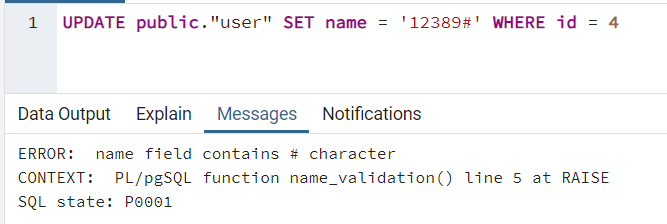
\includegraphics[]{images/validation_1}
        \caption{Trigger raises an exception when user name contains \#}
        \label{fig:db_validation_1}
    \end{figure}

    \begin{figure}[h]
        \centering
        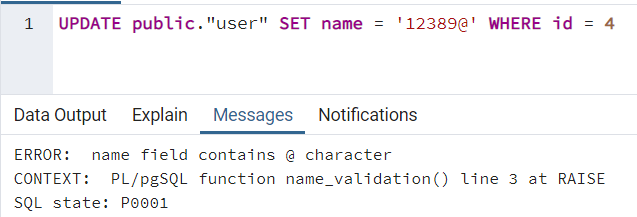
\includegraphics[]{images/validation_2}
        \caption{Trigger raises an exception when user name contains \@}
        \label{fig:db_validation_3}
    \end{figure}
    \begin{figure}[h]
        \centering
        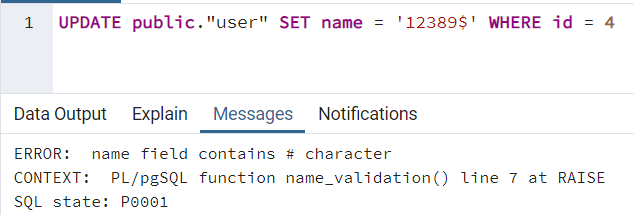
\includegraphics[]{images/validation_dollar}
        \caption{Trigger raises an exception when user name contains \$}
        \label{fig:db_validation_2}
    \end{figure}
\end{center}

\clearpage

\subsection{Function to return user's average place}\label{subsec:function-to-return-user's-average-place}

\texttt{
    CREATE OR REPLACE FUNCTION public.avarage\_user\_ticket\_place(IN "user" "user") \\
    RETURNS integer \\
    LANGUAGE 'sql' \\
    IMMUTABLE \\
    PARALLEL UNSAFE \\
    COST 100 \\
    \\
    \\
    RETURN (SELECT AVG(ticket.place) FROM ticket WHERE ticket.user\_id = "user".id); \\
}

\subsection{Create a function that will return an average user name length for the event by event's name}\label{subsec:select-avarage-user-name-for-the-event-by-event's-name}

\texttt{
    CREATE FUNCTION public.avarage\_users\_name\_length\_for\_event(IN event\_name character varying) \\
    RETURNS numeric \\
    LANGUAGE 'sql' \\
    \\
    \\
    RETURN (SELECT AVG(length) FROM (SELECT LENGTH("name") FROM ( \\
    SELECT DISTINCT "user".name as "name" FROM "event" \\
    INNER JOIN ticket ON ticket.event\_id = "event".id \\
    INNER JOIN "user" ON "user".id = ticket.user\_id \\
    WHERE "event".title LIKE event\_name \\
    ) as select\_user\_names) as select\_length); \\
    \\
    ALTER FUNCTION public.avarage\_users\_name\_length\_for\_event(character varying) \\
    OWNER TO postgres; \\
}

\begin{figure}[h]
    \centering
    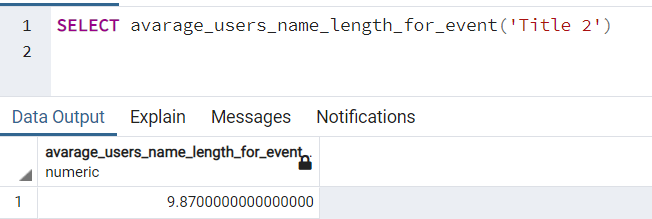
\includegraphics[]{images/avarage_user_name_event}
    \caption{Select average user name for the event by event's name}
    \label{fig:db_average_user_name_length}
\end{figure}

\clearpage
